~\subsection{Organização}
\label{sec:organizacao}

	O ~\textit{uOS} segue uma arquitetura dividida em três camadas, conforme pode ser observado na
	figura ~\ref{fig:arquiteturauOS}.
	
	\begin{figure}[htb]
		\begin{center}
			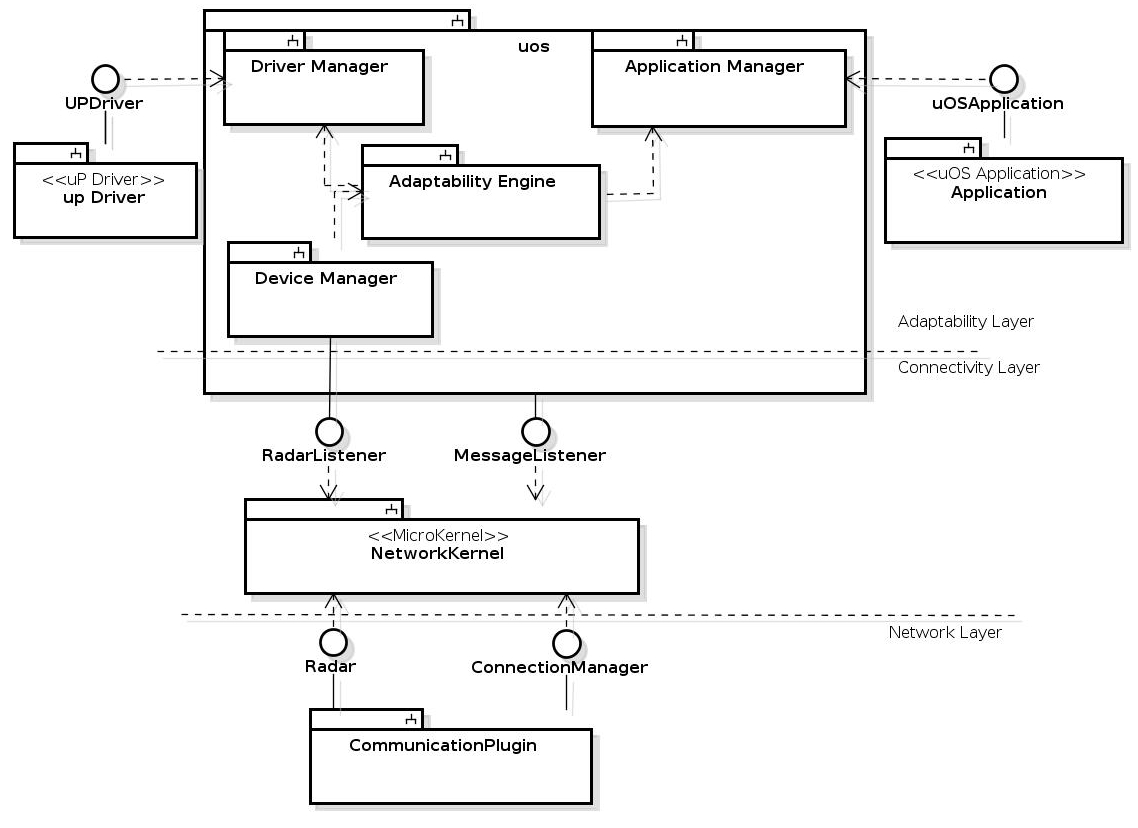
\includegraphics[scale=0.5]{figuras/cap3/uoscamadas.jpg}
		\end{center}
		\caption{Camadas do \textit{uOS}.}
		\label{fig:arquiteturauOS}
	\end{figure}
	
	\begin{enumerate}
	  \item ~\emph{Camada de rede}

		Camada responsável pelo gerenciamento das interfaces de rede do dispositivo, através de
		~\textit{plugins} de redes específicos de acordo com a tecnologia utilizada no acesso. Atualmente,
		são encontrados ~\textit{plugins} para conexões ~\textit{TCP}, ~\textit{UDP},
		~\textit{Bluetooth} e ~\textit{RTP}.
		
		Nesta camada encontra-se os módulos: RADAR e ~\textit{Connection Manager}. O RADAR possui a
		responsabilidade da descoberta de novos dispositivos, por meio de varreduras no ambiente.
		A parte de gerenciameto de conexões entre dispositivos fica sobre responsabilidade do
		~\textit{Connection Manager}.
	  	
	  \item ~\emph{Camada de conectividade}
	  
	 	Responsável pelo gerenciamento das conexões mais internas ao ~\textit{middleware}, ou seja,
	 	gerencia as conexões entre os dispositivos que se comunicam por diferentes tecnologias, como por
	 	exemplo Bluetooth e Ethernet, desta forma não há necessidade de distinção na forma de comunicação
	 	empregada.
	 	
	 	Esta camanda contém os módulos: ~\textit{Radar Listener} e ~\textit{Message Listener}. O
	 	~\textit{Radar Listener} notifica caso um radar encontre um novo dispositivo ou se houve a
	 	saída de um dispositivo do ambiente. O ~\textit{Message Listener} fica responsável pela
	 	transformação dos objetos de acordo com o formato da mensagem ~\textit{uP} recebida, fornecendo
	 	uma visão homogênea das mensgens passadas.
	  
	  \item ~\emph{Camada de adaptabilidade}
	  
		Por fim, esta camada interpreta as operações de mensages recebidas e provê uma comunicação entre
		os ~\textit{drivers} e as aplicações em execução através do módulo ~\textit{Adaptability Engine}.
		Essa comunicação visa selecionar o melhor serviço a ser disponibilizado. 
		
		Além da ~\textit{Adaptability Engine}, possui os outros módulos: ~\textit{Application Manager},
		~\textit{Driver Manager} e ~\textit{Device Manager}. No ~\textit{Application Manager} pode ser
		feito a inclusão e exclusão de aplicações. O ~\textit{Driver Manager} determina o ~\textit{driver}
		para tratar a chamada recebida. O ~\textit{Device Manager} fica responsável pela gestão dos
		dispositivos no ambiente.
		  
	\end{enumerate}